\title{Reference-Guided Merge Tree Maps:\\Quantifying Position--Topology Trade-offs}
\author{Anonymous Authors}\onlineid{0}\vgtccategory{Research}\vgtcinsertpkg
\hypersetup{pdftitle={Reference-Guided Merge Tree Maps: Quantifying Position--Topology Trade-offs}}
\abstract{
Merge tree maps summarize scalar fields through a hierarchy of extrema and their merge relations. Keeping each subtree contiguous can displace features from their projected spatial positions. We present Reference-Guided Merge Tree Maps (RG-MTM), which diagnoses this conflict and constructs maps with an explicit position--topology trade-off. A positional certificate separates interval-packing cost from the additional displacement imposed by hierarchy. Optimal scalar filling for a fixed leaf order preserves extremum values and minimizes labelled pairwise merge-level error, yielding exact attainable frontiers for small trees. RG-MTM-P preserves source merge levels; RG-MTM-R selectively releases contiguity constraints and reports the resulting scalar cost. Across four real temporal sequences and one synthetic sequence comprising 614 frames, both modes improve reference order over shared-input TMTM and ST-MTM baselines. On Storms, the 20\% eligibility setting (R20) reduces P's order error from 3.77\% to 1.16\%, with 1.47\% mean merge-level error; its motion-proxy errors decrease to 19/104 from ST-MTM's 43/104. Independent experiments cover Tangaroa (201 original-grid volumes), Cylinder (102 volumes), one static Nucleon slice, and 21 reconstructed Benzene potential sections. On Tangaroa, R20 reduces P's order error from 9.61\% to 0.019\%, at 14.44\% mean merge-level error. These results quantify the reference alignment gained and scalar connectivity changed by a chosen order, while retaining the source fields for spatial interpretation.
}
\keywords{Temporal scalar fields, merge tree maps, reference-guided layout, positional certificates, merge-level distortion.}
\teaser{
\centering
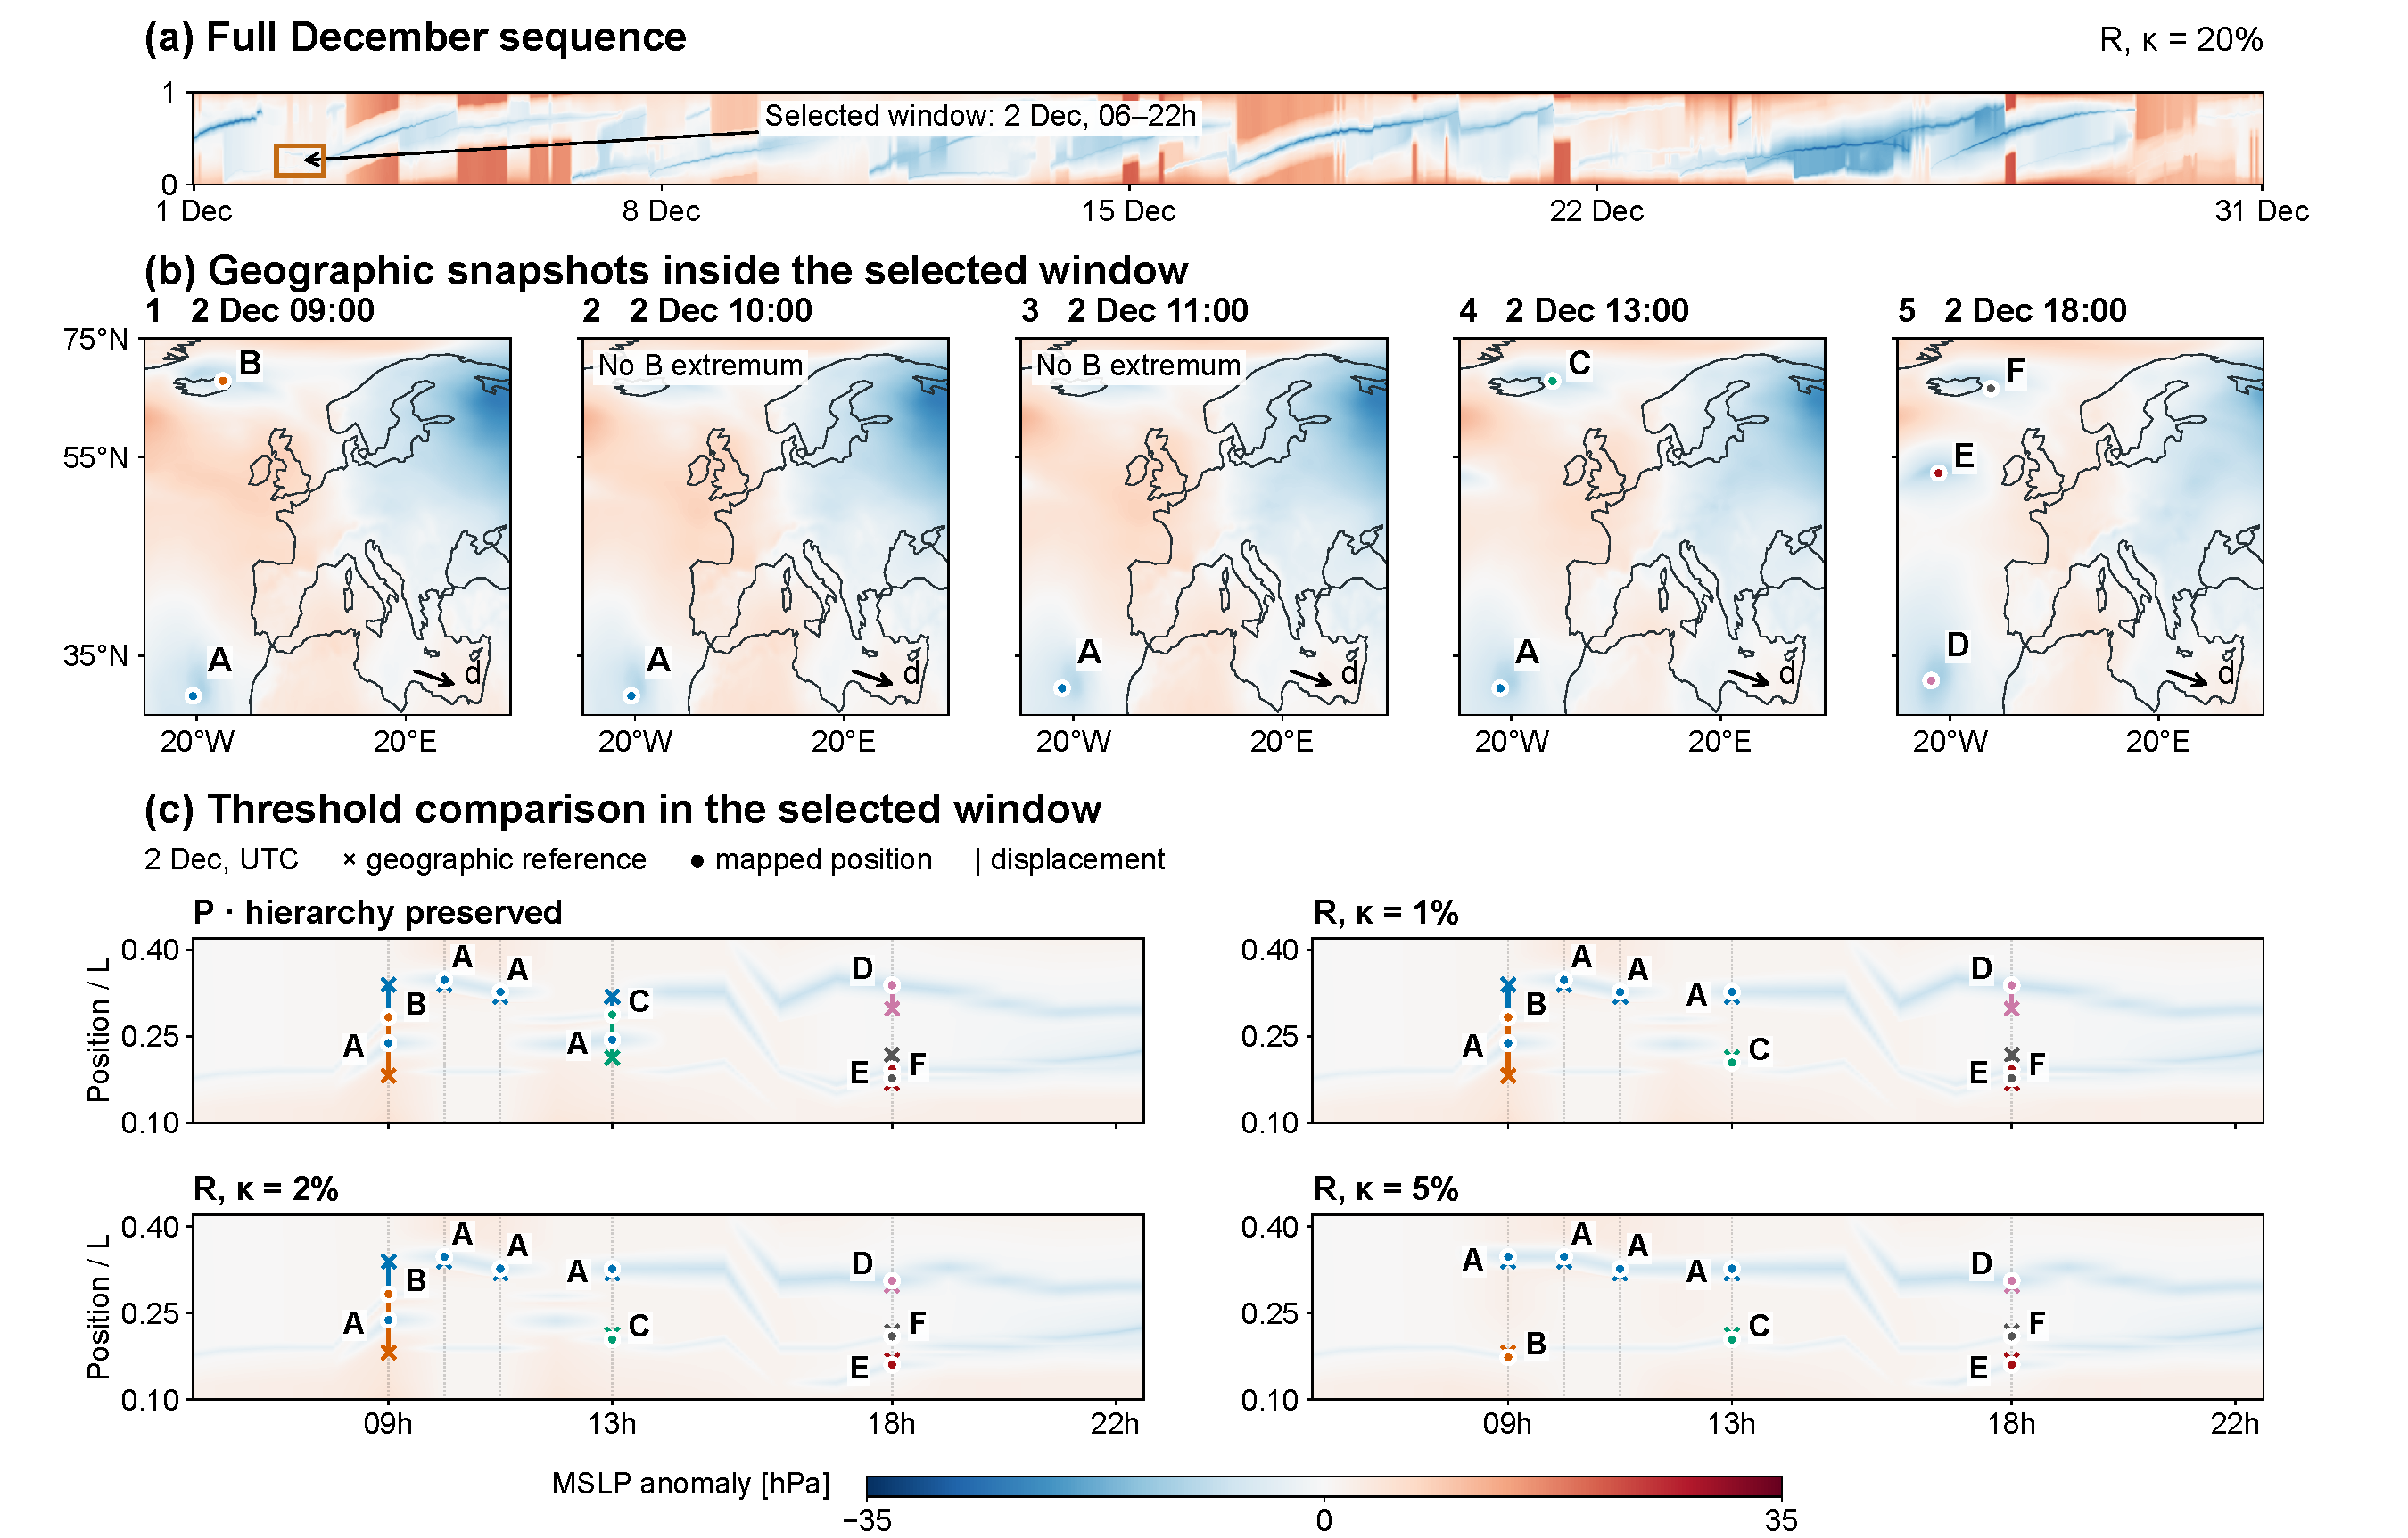
\includegraphics[width=\linewidth]{figures/Fig1.pdf}
\par\smallskip\refstepcounter{figure}\label{fig:teaser}
{\captionfonts\noindent\figurename~\thefigure: RG-MTM-R20 visualization of hourly Storms pressure anomalies over December 1999. (a) All 744 hourly fields are mapped along the data-derived fixed direction $d\approx(0.948,-0.319)$ and linked to five source snapshots. Blue and red encode negative and positive anomalies on a shared $[-35,35]$\,hPa scale. Event names and times follow TMTM~\cite{Koepp:2023:TMTM}; labels identify computed extrema near the reported regions rather than independently validated cyclone tracks. The red dashed outline selects all of 26 December. (b) The 10:00 source field marks $A=130$, $B=113$, and $C=133$; the lower map retains all 24 hourly profiles over the full $[0,1]$ output axis. Solid curves show saved anchors over 00:00--23:00 UTC, with gaps outside saved lifetimes; $C$ exists only from 05:00 to 10:00. Anomalies subtract a centered 192-hour mean; layout uses the RG-MTM $49\times49$ grid and 250\,km smoothing. Display interpolation preserves each hourly profile. This visualization is independent of the 118-frame Storms quantitative evaluation.\par}
}
